\subsection{Results} \label{results}
Four participants reported to have between one and three years of experience with Autodesk Maya, another had between four and six years of experience and the last had seven or more years of experience. Only one participant had more than one year of experience with Unity, another had between six and twelve months of experience with it, the rest reported to have less than six months of experience.
When asked if they \textit{'felt empowered using the tool'}, 2/6 participants \textit{strongly agreed} and 4/6 participants \textit{agreed}.

The coded data gathered from video analysis shows that The number of events tagged with \textit{confusion} and \textit{problem} in the task and creative-phase can be seen in Figure \ref{fig:codedgraph}. In the task-phase, 23 events was tagged as confusion and 15 as problem. In the creative-phase, 7 events was tagged as confusion and 4 as problem. This is an increase of 53.4\% and 57.8\% for confusion and problem, respectively.

\begin{figure}[htbp]
\centering
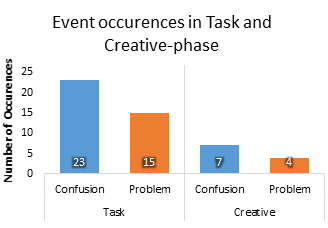
\includegraphics[width=0.45\textwidth]{Pics/codedgraph2}
\caption{Number of occurrences for confusion and problem in both the task and creative-phase.}
\label{fig:codedgraph}
\end{figure}

When asked if the participants felt empowered using the tool, four participants agreed while the remaining two strongly agreed. When asked if the they felt restricted when using the tool, five participants disagreed while the remaining participant strongly disagreed. To find out how efficient the participants felt using our tool, we asked them if they felt they got the tasks done quick, four participants agreed and two strongly agreed. To find out how effective the participants felt using our tool, we asked them if they felt the tool allowed them to complete the tasks well, three participants agreed and three strongly agreed.
When asked about the preview features, five participants found them very useful, and one found it somewhat useful. For the participants' favorite feature for adjusting camera positions, four named 'Be the camera' and two named 'Snapshot' as their favorite. Furthermore, three participants noted the 'Be the camera' feature as their overall favorite while the 'Slider Preview' was the favorite for the other three participants. 